\chapter{Desarrollo del proyecto}

En este capítulo se describe el desarrollo del proyecto

\section{Direcciones de grupo y objetos de comunicación}
\label{sec:dir_grup}

Al utilizar el estándar de programación de KNX, será necesaria la creación de las direcciones de grupo del sistema, cuya función principal será la de actuar como nexo de comunicación entre los diferentes objetos de comunicación con los que cuentan los módulos. Todos los objetos de comunicación cuentan con seis \textit{flags} distintos seleccionables en función de la ocupación que vayan a desarrollar, a saber:
\begin{itemize}
\item \textit {C-flag}: es el \textit{flag} de comunicación (\textit {Communication}), y tal y como indica su nombre, su función será la de abrir y permitir el canal de comunicación hacia ese objeto de comunicación del módulo. Por lo general, es un \textit{flag} que se encuentra activo en prácticamente todos los objetos, y solo será deshabilitado en situaciones muy concretas en las que su no actuación sea crítica.
\item \textit {R-flag}: es el \textit{flag} de lectura (\textit {Read}), y permite al objeto de comunicación ser consultado por su valor, como si de una variable de programación se tratase. Este \textit{flag} se encuentra activo principalmente en aquellos objetos que devuelven el estado de un parámetro del sistema, como por ejemplo, el estado en que se encuentra una de las salidas de un actuador ON/OFF. Cuando otro objeto trate de comunicarse con él, contestará con el valor actual en el que se encuentra, 0 ó 1, siguiendo con el ejemplo anterior, pero pudiendo ser un valor de la posición en porcentaje de apertura de una ventana o el valor de la temperatura de consigna establecida en ese momento en el módulo. Son usados para representar el estado de las variables en una interfaz gráfica para poder ser consultados por el usuario.
\item \textit {T-flag}: se trata del \textit{flag} de transmisión (\textit {Transmit}), el cual cuanta con bastante similitud con el \textit {R-flag}, con la salvedad de que este objeto no espera a ser consultado para enviar su valor, sino que lo enviará siempre que se produzca un cambio de valor en él. Un ejemplo de este comportamiento, lo podemos encontrar en los objetos de comunicación que reciben el estado de un sensor, enviando la actualización de su valor en cuanto que esta se produce.
\item \textit {W-flag}: es el \textit{flag} de escritura (\textit {Write}), y será aquel que recibe el valor de la variable desde los actuadores físicos, los \textit{R-flag} o los \textit{T-flag} y les permite sobrescribir su valor. Esto es muy útil a la hora de que exista varios puntos de control de un mismo elemento y todos conozcan y se encuentren con el mismo valor, actuando a su vez sobre los elementos hardware de la instalación. Por ejemplo, al ejecutar una pulsación sobre un interruptor, este \textit{flag} permitirá que el objeto de comunicación modifique su valor de 0 a 1, o viceversa, enviando la orden al actuador para que abra o cierre el relé correspondiente.
\item \textit {U-flag}: es el \textit {flag} de actualización (\textit {Update}), cuya misión es simplemente la de buscar de manera continua algún tipo de modificación en los estados, para así modificar su valor de manera automática. Estos \textit{flags} no suelen ser muy utilizados en objetos de comunicación que cuenten con \textit {R-flag} o \textit {T-flag}, ya que se producen bastantes errores al leerse a sí mismos, provocando bucles de realimentación de estado durante tiempos indefinidos, ocupando la línea de comunicación del bus, dando lugar a un colapso en ella. Se suelen activar con \textit {W-flag}, permitiendo así su autoreescritura en cuanto se produce algún cambio en sus asociaciones.
\item \textit {I-flag}: se trata del \textit {flag} que permite al objeto de comunicación adoptar un valor al inicio (\textit {Initialization}) de su funcionamiento o tras una caída en la tensión del bus o cualquier otro problema relacionado con la perdida de comunicación del módulo con el resto del sistema.
\end{itemize}
Todos estos \textit {flags} pueden ser activados en todos y cada uno de los objetos de comunicación, aunque su activación no implica que realmente vaya a cumplir con esa funcionalidad, ya que también se requiere que el hardware de su módulo pueda físicamente ejecutarlo. Un ejemplo del comportamiento más usual en las comunicaciones con protocolo KNX lo vemos representado en la Imagen \ref{fig:diag_flags},  donde podemos ver que el objeto de comunicación textit {ON/OFF Luz Cocina} se inicializa con el valor 0 preprogramado gracias a su \textit {I-flag} y se envía la orden al actuador por tener el textit {W-flag} activo. Una vez que el actuador, en este ejemplo, abra el relé, el objeto de comunicación textit {STD ON/OFF Luz Cocina} recoge el estado en que se encuentra esa salida debido a que este objeto tiene en funcionamiento su \textit {R-flag}. De este objeto de comunicación se harán lecturas de ese valor desde otros objetos de comunicación que se encuentren ligados a él en la misma dirección de grupo, como pueden ser los LEDs de dos pulsadores y un icono de la interfaz gráfica que representan este estado, que gracias a su \textit {W-flag}, actualizarán su valor a 0.\\\\
Si ahora se pulsase el pulsador P1, este escribiría un 1 en el objeto de comunicación textit {ON/OFF Luz Cocina}, lo que provocaría que el actuador cerrase el relé, permitiendo la circulación de la corriente y por tanto, el encendido de la bombilla. En ese momento, el objeto de comunicación textit {STD ON/OFF Luz Cocina} detecta el cambio de estado de la salida del actuador, y actualiza su valor a 1, volviendo a permitir que, no solo P1, si no también P2 y la pantalla, actualicen su estado y enciendan sus LEDs informativos y el icono cambiase a su representación de luz encendida. De esta manera el usuario es capaz de conocer el estado de un elemento de manera remota. Si ahora se diese el caso de que se pulsase el pulsador P2 o se actuase desde la pantalla, al conocer el estado en que se encuentra actualmente la luz, enviarán el valor contrario mediante una acción de textit {switch}, en este caso 0, volviendo a actuar sobre el actuador pero a la vez informando al resto de módulos del estado de ese elemento, tal y como sucedió al actuar sobre P1.
 \begin{center}
\begin{figure}[H]
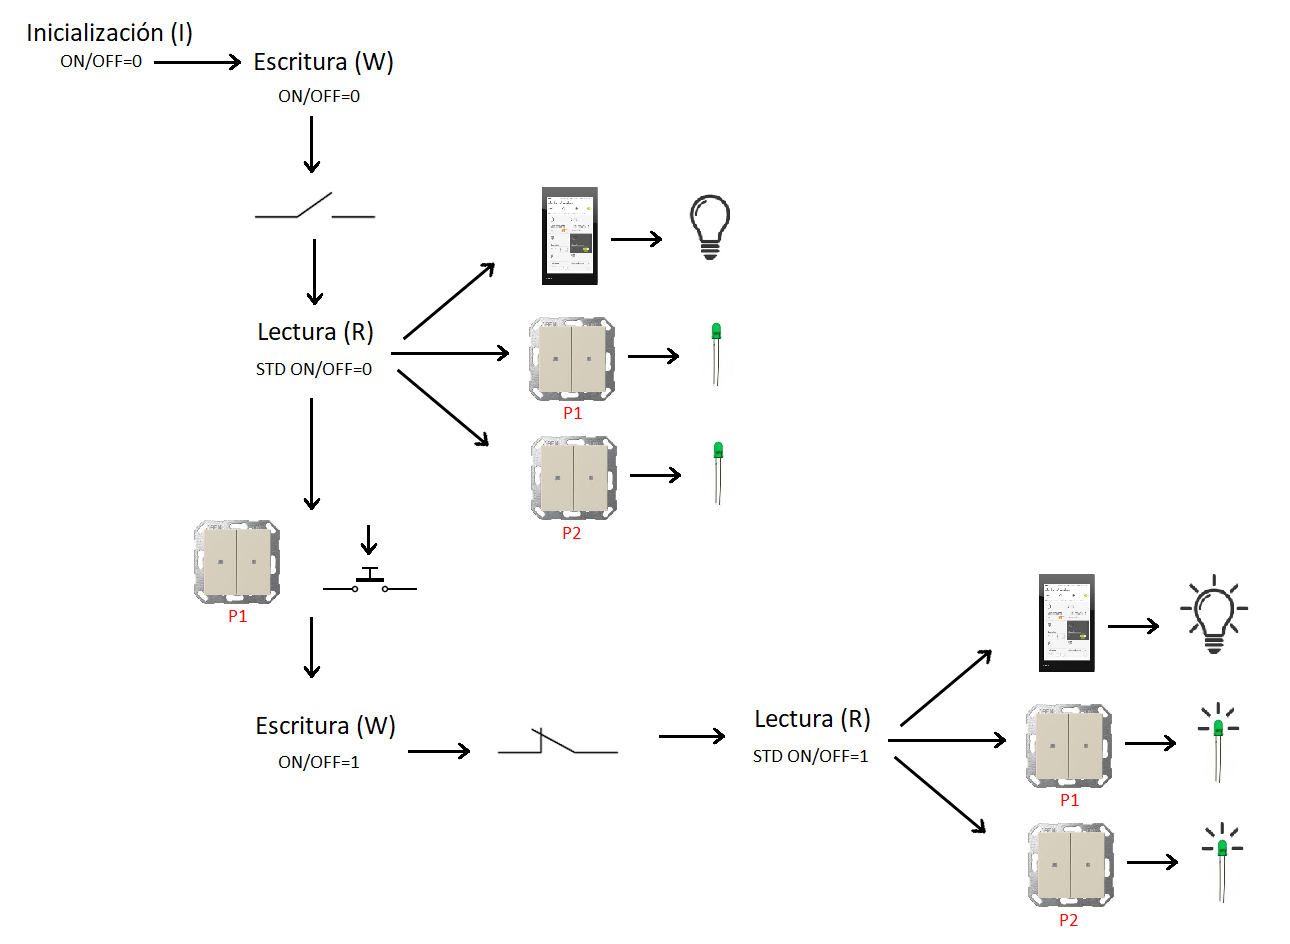
\includegraphics[width=1.15\textwidth]{figures/diag_flags.png}   
\caption{Diagrama uso de flags}
\label{fig:diag_flags}
\end{figure}
\end{center}
Como se comentaba al comienzo de este capítulo, los objetos de comunicación de los mecanismos se comunican entre sí al linkarse a la misma dirección de grupo, como es el caso de los LEDs de los pulsadores y el icono de la pantalla, que están linkados a la dirección de grupo denominada textit {ON/OFF Luz Cocina}. Estas direcciones han de ser creadas por el programador en función de las tareas y acciones que desee realizar en la instalación. Para una mayor organización, el software ETS5 ofrece tres niveles de dirección de grupo: el principal, que da información acerca de que sección se controla, uno intermedio, que anuncia que funcionalidad se ejecuta, y finalmente las propias direcciones de grupo, que llevarán el nombre concreto del efector y la función que utiliza. Siguiendo con el ejemplo de la Imagen \ref{fig:diag_flags},  el nivel superior llevaría el nombre de textit {Iluminación} con el número 1, el intermedio textit {ON/OFF} con la identificación 1/1, y finalmente, y tal como se comentó, la dirección de grupo será nombrada como textit {ON/OFF Luz Cocina}, con tipificación 1/1/1. De esta manera, se establece una jerarquía organizativa que permite a los instaladores o incluso programadores futuros que modifiquen el proyecto, localizar las direcciones de grupo de manera más intuitiva y sencilla.
\newpage
En este proyecto se ha creado la siguiente jerarquía de organización para contener todos los objetos de comunicación que van a ser utilizados durante el funcionamiento de la instalación:

\begin{multicols}{2} 
\begin{flushleft} 
\begin{itemize}
\item{0 General}
\begin{itemize}
\item{0/1 Escenas}
\item {0/2 Parámetros del sistema}
\end{itemize} 
\end{itemize} 
\vspace{1.5cm}
\end{flushleft} 

\begin{flushright}  
\begin{itemize}
\item{1 Iluminación}
\begin{itemize}
\item{1/1 ON/OFF}
\item{1/2 STD ON/OFF}
\item{1/3 DIMMING}
\item{1/4 VALOR DIMMING}
\item{1/5 STD VALOR DIMMING}
\end{itemize} 
\end{itemize} 
\end{flushright} 
\end{multicols} 

\begin{multicols}{2} 
\begin{flushleft} 
\begin{itemize}
\item{2 Persianas, Proyector y Puerta}
\begin{itemize}
\item{2/1 UP/DOWN}
\item{2/2 STEP/STOP}
\item{2/3 VALOR}
\item{2/4 STD VALOR}
\item{2/5 TIMBRE}
\item{2/6 PUERTA}
\end{itemize} 
\end{itemize} 
\vspace{0.5cm}
\end{flushleft} 

\begin{flushright} 
\begin{itemize}
\item{3 Climatizacion}
\begin{itemize}
\item{3/1 ON/OFF}
\item{3/2 STD ON/OFF}
\item{3/3 MODO CLIMA}
\item{3/4 STD MODO CLIMA}
\item{3/5 TEMP CONSIGNA}
\item{3/6 STD TEMP CONSIGNA}
\item{3/7 TEMP REAL}
\end{itemize} 
\end{itemize} 
\end{flushright} 
\end{multicols} 

\begin{multicols}{2} 
\begin{flushleft} 
\begin{itemize}
\item{4 Variables climatizacion}
\begin{itemize}
\item{4/1 POS REJILLA}
\item{4/2 STD POS REJILLA}
\item{4/3 VEL FAN}
\item{4/4 STD VEL FAN}
\item{4/5 MODO FAN}
\item{4/6 STD MODO FAN}
\item{4/7 STD VENTANA}
\end{itemize} 
\end{itemize} 
\end{flushleft}

\begin{flushright} 
\begin{itemize}
\item{5 Consumo}
\begin{itemize}
\item{5/1 SOLICITUD}
\item{5/2 CAUDAL AGUA (l/h)}
\item{5/3 CAUDAL GAS (m3/s)}
\item{5/4 POTENCIA (kW)}
\item{5/5 ENERGIA (kW•h)}
\item{5/7 FECHAS}
\end{itemize} 
\end{itemize} 
\end{flushright} 
\end{multicols} 

\begin{multicols}{2} 
\begin{flushleft} 
\begin{itemize}
\item{6 CO\textsubscript{2} y Recuperador}
\begin{itemize}
\item{6/1 LIMITES CO2}
\item{6/2 ON/OFF FAN CO2}
\item{6/3 STD ON/OFF FAN CO2}
\item{6/4 VEL FAN CO2}
\item{6/5 STD VEL FAN CO2}
\item{6/6 MEDIDA CO2}
\end{itemize} 
\end{itemize} 
\end{flushleft}

\begin{flushright} 
\begin{itemize}
\item{7 Detectores y efectores}
\begin{itemize}
\item{7/1 ON/OFF ELECT. VALV.}
\item{7/2 STD ELECT. VALVULAS}
\item{7/3 SIRENA HUMO}
\item{7/4 STD SIRENA HUMO}
\item{7/5 STD DETECTORES}
\end{itemize} 
\end{itemize} 
\end{flushright} 
\end{multicols} 

\begin{flushleft} 
\begin{itemize}
\item{8 Centralizados}
\begin{itemize}
\item{8/1 ILUMINACION}
\item{8/2 CLIMA}
\item{8/3 PERSIANAS}
\end{itemize} 
\end{itemize} 
\end{flushleft}

A continuación, se realiza una breve explicación de que significa cada una de estas direcciones de grupo de nivel medio para facilitar la comprensión de esta clasificación:
\begin{itemize}
\item Estados: por norma general, todas las direcciones de grupo de acciones llevan asociada una dirección de estado, nombradas como STD y que contienen el mismo tipo de variables, para realizar la lectura del estado del efector que ha sido modificado. Serán del mismo tamaño que la acción a la cual se encuentran referenciadas.
\item Dimming: este tipo de datos será el encargado de enviar los telegramas que indican a los mecanismos si deben “subir” o “bajar”, como es el caso de la posición de una persiana o el de regular la intensidad de una bombilla. Cuentan con un tamaño de 4 bits.
\item Up/Down: envía la orden de subir o bajar mediante el envio de un 0 ó un 1, por lo que su longitud de paquete será de 1 bit.
\item Step/Stop: permite enviar un telegrama que indique al mecanismo que debe para en su regulación o dar un “paso” preajustado (normalmente del 12.5\% del total), tanto de “subida” como de “bajada”. Su tamaño es de 1 bit.
\item Valor dimming o posición: esta dirección permitirá al usuario enviar un valor porcentual concreto al elemento regulable, para establecer su nivel de “subida” y “bajada” en una posición concreta. Por ejemplo, permite enviar un “50\%” a una lámpara, para que se regule a la mitad de su máxima intensidad lumínica. En esta ocasión, el tamaño de esta variable será de 1 byte, ya que se requerirá mayor espacio para enviar el valor del porcentaje con una precisión de 1/256.
\item Temperaturas: esta clase de direcciones permitirá transmitir valores de tipo temperatura, que contarán con 2 bytes de memoria para permitir los valores decimales, ofreciendo así la posibilidad de regular con mayor precisión las temperaturas deseadas en la vivienda.
Valores de lectura: estos parámetros son utilizados para hacer lecturas de los sensores implementados en el sistema. Debido a la gran variedad de estos, no poseen un tamaño fijo y su valor fluctuará desde 1 bit, como en el caso de un sensor de detección de ventana abierta/cerrada, hasta un máximo de 4 bytes, como en la lectura del caudal de gas.
\item Centralizados: este tipo de dirección permite agrupar diversos objetos de comunicación para que los mecanismos se comporten todos de la misma manera en el mismo instante. Su funcionalidad es totalmente abierta, y por tanto su tamaño dependerá de la acción que se ejecute. Los centralizados son utilizados en este proyecto para realizar un apagado general del sistema de iluminación (1bit) o para hacer un control sobre la posición de todas las persianas (1 byte), permitiendo así situarlas todas en la misma posición proporcional.
\item Escenas: estas direcciones tienen una lógica similar a la de los centralizados, con la salvedad de que estos permiten enviar diferentes órdenes a los mecanismos de manera simultánea. Una escena que se ha programado en este proyecto, recibe el nombre de “Salir de casa”, y en ella se ejecuta el apagado de todas las luces de la vivienda, se bajan todas las persianas y se desactiva el recuperador de CO\textsubscript{2}.
\end{itemize} 

\section{Programación de los mecanismos}

Una vez explicada la base de trabajo de la programación, en este capítulo se pasará a comentar el linkado que se ha establecido entre los diferentes objetos de comunicación de los módulos instalados en la vivienda y las direcciones de grupo creadas y comentadas con anterioridad. También se detallarán los bloques lógicos creados para satisfacer los requisitos del cliente en aquellas ocasiones que los objetos de comunicación predefinidos de los módulos no llegan al alcance requerido de precisión o funcionalidad, y por tanto, es necesaria la implementación de una programación complementaria. Los bloques lógicos son una variedad de funciones del tipo \textit {drag and drop} que ofrece el servidor X1 y permite crear entramados complejos de pautas de funcionamiento mediante la asociación de \textit {“cajas lógicas”} que manipula, transforma o asocia direcciones de grupo. En esta sección se explicará en detalle también la lógica aplicada durante el diseño de estos bloques lógicos.

\subsection{Iluminación} Esta sección entrelazará los pulsadores domóticos con los actuadores, tanto binarios como reguladores, a través del bus KNX para poder actuar sobre el sistema de iluminación de la vivienda a través de la dirección de grupo ON/OFF. A las teclas de los pulsadores que se encargarán del apagado, encendido y regulación de luminarias, se les ha otorgado la funcionalidad de conmutación con aplicación de tipo \textit {“switch”}, permitiendo así el envío del valor binario adecuado (contrario al existente en el momento) al accionar el pulsador. Por otro lado, se han programado ambas clases de actuadores para que en caso de caída de tensión en el bus, recuperen de su \textit {stack} de memoria el último valor en el que se encontraban las luces previamente. \\\\
El funcionamiento básico de esta sección hace de su programación una tarea sencilla y sin ningún tipo de complejidad, pero por solicitud del cliente ha sido necesario implementar un complejo bloque lógico para lograr controlar las lámparas dimmeables desde el único punto de los pulsadores KNX. El funcionamiento esperado sigue las siguientes pautas: con una pulsación larga, la lámpara comienza a aumentar su intensidad lumínica si la acción durante la última pulsación larga había sido reducir el valor lumínico. Por el contrario, si la última acción había sido aumentar de tensión, al realizar una pulsación larga, debe comenzar a descender su intensidad. \\
Por otro lado, y en cuanto a la pulsación corta, si se da mientras no se esté ejecutando ninguna regulación: si la luz se encuentra encendida, pasará a estar apagada, mientras que si se encontraba apagada, regulará de manera automática y progresiva la intensidad lumínica hasta el valor guardado en el \textit {stack} de memoria en el momento de parar la regulación.
\newpage
 El diagrama de bloques diseñados en el módulo X1 es el siguiente:
 \begin{center}
\begin{figure}[H]
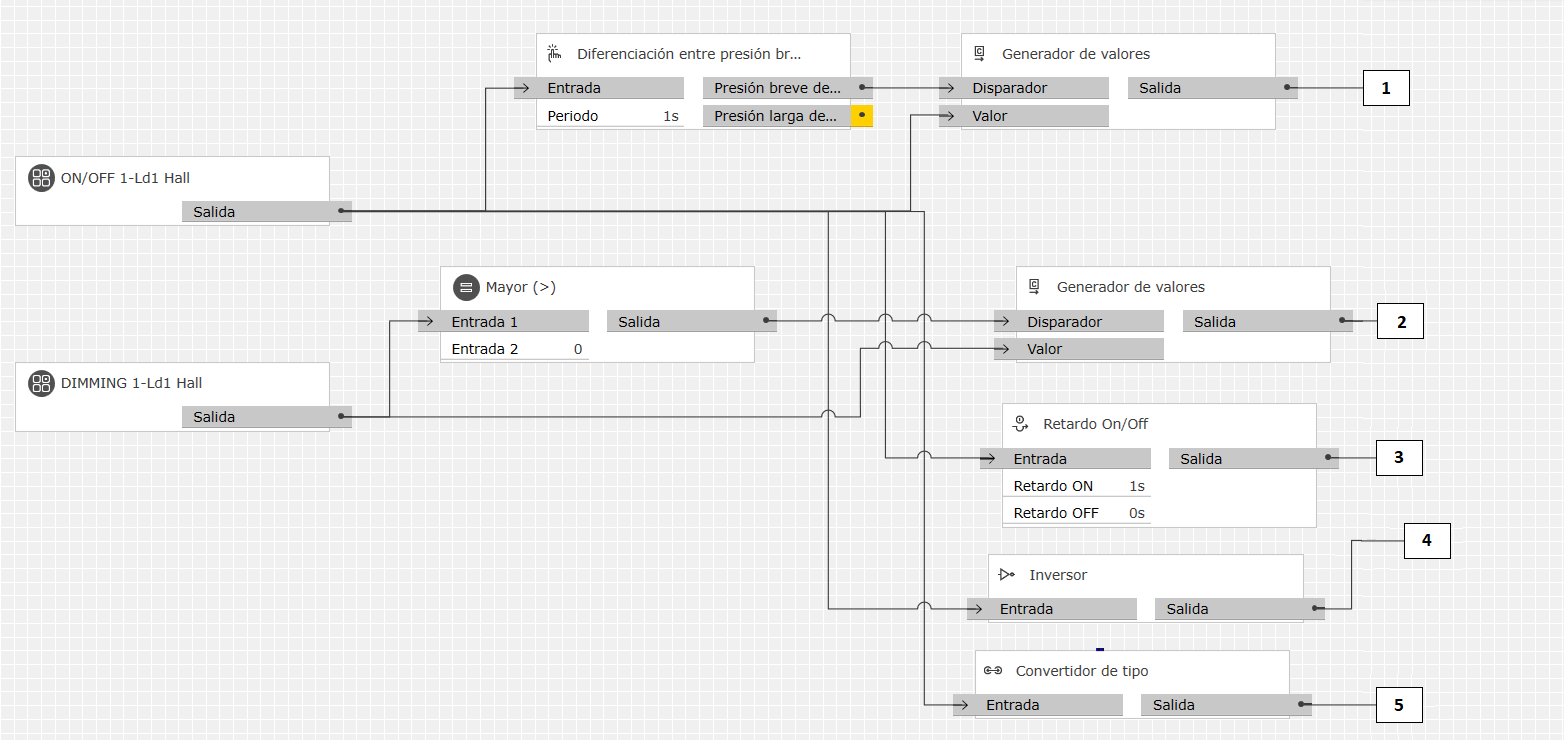
\includegraphics[width=1.05\textwidth]{figures/log_dimm_izq.png}   
\caption{Módulo lógico DIMMER (1ª Parte)}
\label{fig:log_dimm_izq}
\end{figure}
\end{center}
 \begin{center}
\begin{figure}[H]
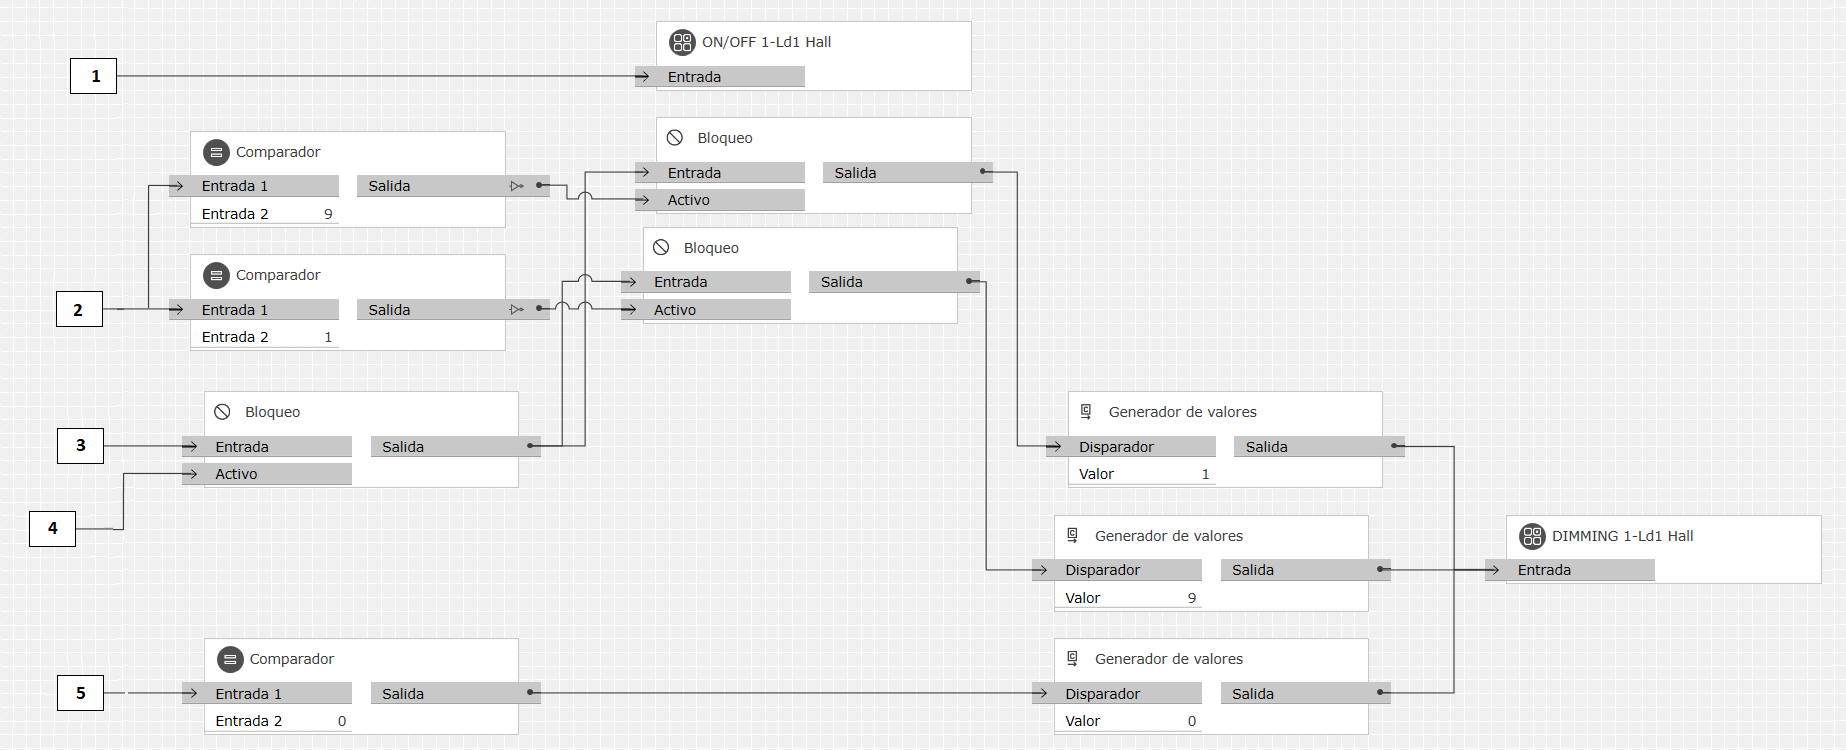
\includegraphics[width=1.05\textwidth]{figures/log_dimm_der.png}   
\caption{Módulo lógico DIMMER (2ª Parte)}
\label{fig:log_dimm_der}
\end{figure}
\end{center}
En él podemos encontrar dos entradas de datos: la señal de ON/OFF de la luminaria y la orden de DIMMER, que atacarán a sus homologos de las salidas, una vez realizadas todas las secuencias del bloque lógico, que a continuación será descrito: 
\newpage
Por un lado, la señal de ON/OFF se envía a un bloque lógico capaz de diferir entre una pulsación larga de una corta, preestableciendo el valor que las diferencia durante su programación, en este caso, de un segundo. Este bloque ha sido programado para que únicamente se obtenga una señal de salida de valor “1” cuando la pulsación que es detectada es breve, y es enviada al disparador de un bloque Generador de valores. Este bloque tiene la función de que en el momento que recibe un “1” por su puerto “Disparador”, envía el valor recibido por su puerto “Valor”, que en este caso, es la propia señal de ON/OFF de la entrada. Este valor será recibido por un bloque de salida, que es el encargado de modificar el valor de la propia dirección de grupo ON/OFF de la lámpara.
\begin{center}
\begin{figure}[H]
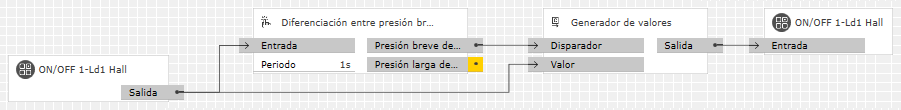
\includegraphics[width=1.15\textwidth]{figures/log_dimm_b1.png}   
\caption{Módulo lógico DIMMER: bloque 1}
\label{fig:log_dimm_b1}
\end{figure}
\end{center}
Con estos módulos lo que se logra simular es el encendido y apagado de la bombilla regulada desde el actuador de regulación al hacer una pulsación corta sobre el pulsador domótico.\\\\
A continuación, encontramos la segunda entrada, en este caso apuntando hacia la dirección de grupo DIMMING, la cual, en primera instancia, entrará a un bloque lógico Comparador. Este bloque se ha configurado para que su salida sea un “1” cuando el valor de entrada sea mayor que 0. Tanto para el valor de subida como de bajada, el valor de este telegrama será mayor de 0, respectivamente y en valores binarios, 101 y 001. En estos dos  casos, la salida del comparador será un “1”, que irá direccionado al puerto “Disparador” de otro bloque Generador de valores, cuyo valor de salida al activarse será el propio valor de la entrada de DIMMER. \\ Este valor será enviado a dos bloques Comparadores, uno programado para identificar unos y otro para nueves, cuyas salidas irán invertidas y direccionadas a la entrada de activación de un módulo de Bloqueo cada una. Estos módulos tienen un funcionamiento bastante sencillo e intuitivo: actúan como de buffer de datos, que entran por su puerto “Entrada”, siempre que reciban un “0” por su puerto “Activo”, puesto que si por el contrario reciben un “1”, bloquearan el envío de ese valor. 
 \begin{center}
\begin{figure}[H]
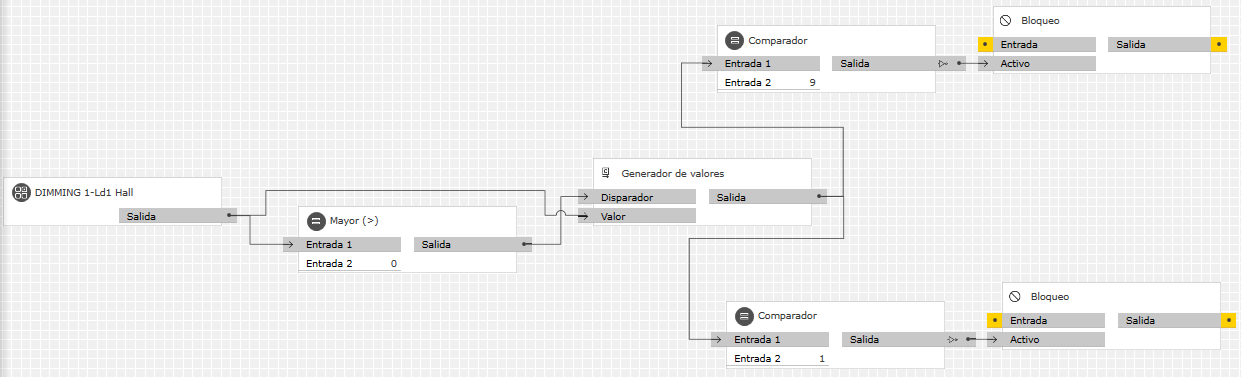
\includegraphics[width=1.15\textwidth]{figures/log_dimm_b2.png}   
\caption{Módulo lógico DIMMER: bloque 2}
\label{fig:log_dimm_b2}
\end{figure}
\end{center}
Por otro lado, los valores que se envían una vez que estos módulos de Bloqueo son desactivados provienen del tratamiento de la entrada ON/OFF. Esta señal en primer lugar pasará por un bloque lógico de Retardo ON/OFF, el cual permite seleccionar el tiempo de retardo del envío de las señales de ON/OFF, que en esta ocasión únicamente se ha establecido en 1 segundo para el ON, manteniendo el envío instantáneo para el OFF. A continuación, estos valores irán a la entrada de otro módulo de Bloqueo, cuya señal de activación es el valor invertido de la propia señal ON/OFF al pasar a través de un bloque Inversor, logrando así únicamente transmitir el “1” generado al activar la señal de ON/OFF, siendo este “1” las señales de entrada y valor a transmitir de los módulos de Bloqueo activados por los bloques Comparadores de unos y nueves mencionados anteriormente, cuya función era la de activarlos y desactivarlos. Una vez que estos bloques se encuentran desactivados y permiten el paso del valor, este se dirige a la entrada disparador de un Generador de señales, uno por cada módulo de Bloqueo, que transmitirán un uno o un nueve a la salida de DIMMING, según cuál de ellos sea activado.
 \begin{center}
\begin{figure}[H]
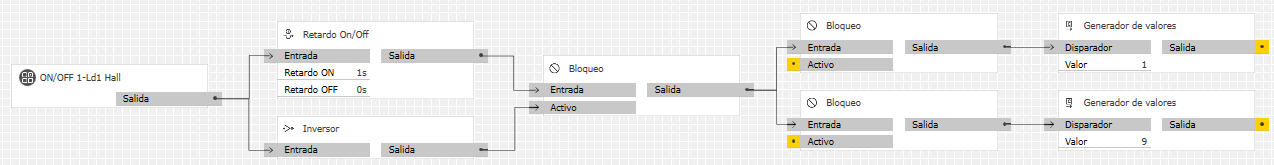
\includegraphics[width=1.15\textwidth]{figures/log_dimm_b3.png}   
\caption{Módulo lógico DIMMER: bloque 3}
\label{fig:log_dimm_b3}
\end{figure}
\end{center}
En último lugar, la señal de ON/OFF volverá a ser utilizada, siendo en primer lugar por un bloque Convertidor de tipo, configurado para obtener a su salida un valor binario de esta entrada. Una vez convertido, este valor pasará a un bloque Comparador programado para  contrastar si el valor recibido es un “0”, y enviar un “1” al puerto disparador de un bloque Generador de valores, que enviará un cero a la salida de DIMMING una vez se dispare. 
 \begin{center}
\begin{figure}[H]
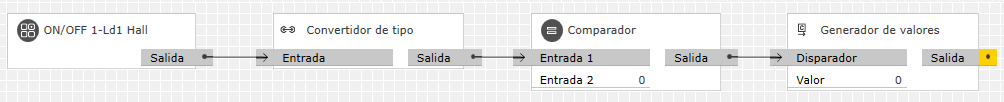
\includegraphics[width=1.15\textwidth]{figures/log_dimm_b4.png}   
\caption{Módulo lógico DIMMER: bloque 4}
\label{fig:log_dimm_b4}
\end{figure}
\end{center}
Con la unión de los paquetes lógicos 2, 3 y 4 lo que se logra es hacer un envío cíclico y ordenado de los valores de dimming de subida y bajada de tensión, que serán alternados a través del uso de los paquetes 2 y 3, que enviarán alternativamente los valores “1” y “9” correspondientes con la orden de bajada y subida respectivamente, mientras que el valor “0” será enviado siempre a la salida de DIMMING cuando se produzca en la entrada ON/OFF, simplemente para que esa dirección de grupo actualice su estado de cara al próximo proceso de regulación de esa lámpara o bien para actualizar su estado en las interfaces gráficas que utiliza el cliente.
 \begin{center}
\begin{figure}[H]
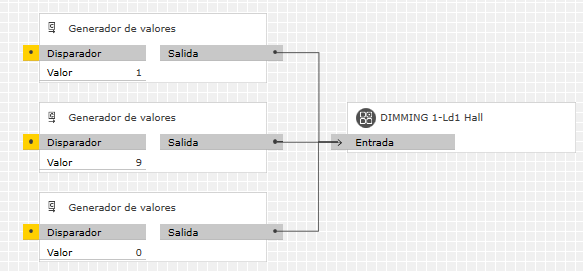
\includegraphics[width=0.95\textwidth]{figures/log_dimm_b5.png}   
\caption{Módulo lógico DIMMER: bloque 5}
\label{fig:log_dimm_b5}
\end{figure}
\end{center}
En la Imagen \ref{fig:prog_dim} del Anexo~\ref{aped.B} se muestra los linkados necesarios en las direcciones de grupo de una luminaria de tipo regulable, ya que engloba todas las variables utilizados en una de clase ON/OFF.

\subsection{Persianas/ventanas}Como ya se comentó en la sección \ref{sec:dir_grup}, las persianas y ventanas harán uso de 4 direcciones de grupo: UP/DOWN, STEP/STOP, VALOR y STD VALOR, que se encuentran linkadas entre los pulsadores y el actuador a través del bus. Las salidas del actuador destinadas a realizar esta función de regulación, han sido configuradas con el modo persiana, del tipo persiana enrollable o toldo. Una vez aplicado este modo de funcionamiento a las salidas del actuador, se permite el ajuste de varios de los parámetros, como es el caso de los tiempos de actuación de cada persiana: se deberá cronometrar los tiempos de bajada y subida de estas, para que así, el sistema sea capaz de enviar un valor porcentual del nivel de bajada en función del tiempo que se haya encontrado en funcionamiento, ya que el motor de la persiana no cuenta con ningún control de posición absoluto en su encoder o sistema de cuantificación de movimiento. Con la intención de dar un ajuste más fino, se implementa un parámetro que permite añadir un tiempo adicional al tiempo de subida de la persiana, para así compensar las diferencias de tiempo de recorrido que pueden encontrarse debido al elevado peso de las lamas que componen las persianas. Estas salidas han sido programadas para enviar una orden de paro tras la caída de tensión del bus, con la intención de evitar daños en su estructura, que podrían venir causados por el desconocimiento de la posición real de las persianas por parte del sistema y hacer que estas se descuelguen o se salgan de sus rieles en el caso de que los finales de carrera no se encuentren operativos o bien ajustados.\\\\
Finalmente, la programación de una ventana o persiana controlada domóticamente se vería tal y como se muestra en la siguiente Imagen \ref{fig:prog_dim} del Anexo~\ref{aped.B}, donde se aprecia una captura de pantalla de la programación en el software ETS5.

\subsection{Climatización}Esta sección se trata de la que posee una mayor complejidad a la hora de programar debido a que debe integrar los numerosos módulos que la componen, y por ello, se ha creado el siguiente esquema simplificado para facilitar su comprensión en lugar de realizar una captura de pantalla a los linkados en el ETS5:
 \begin{center}
\begin{figure}[H]
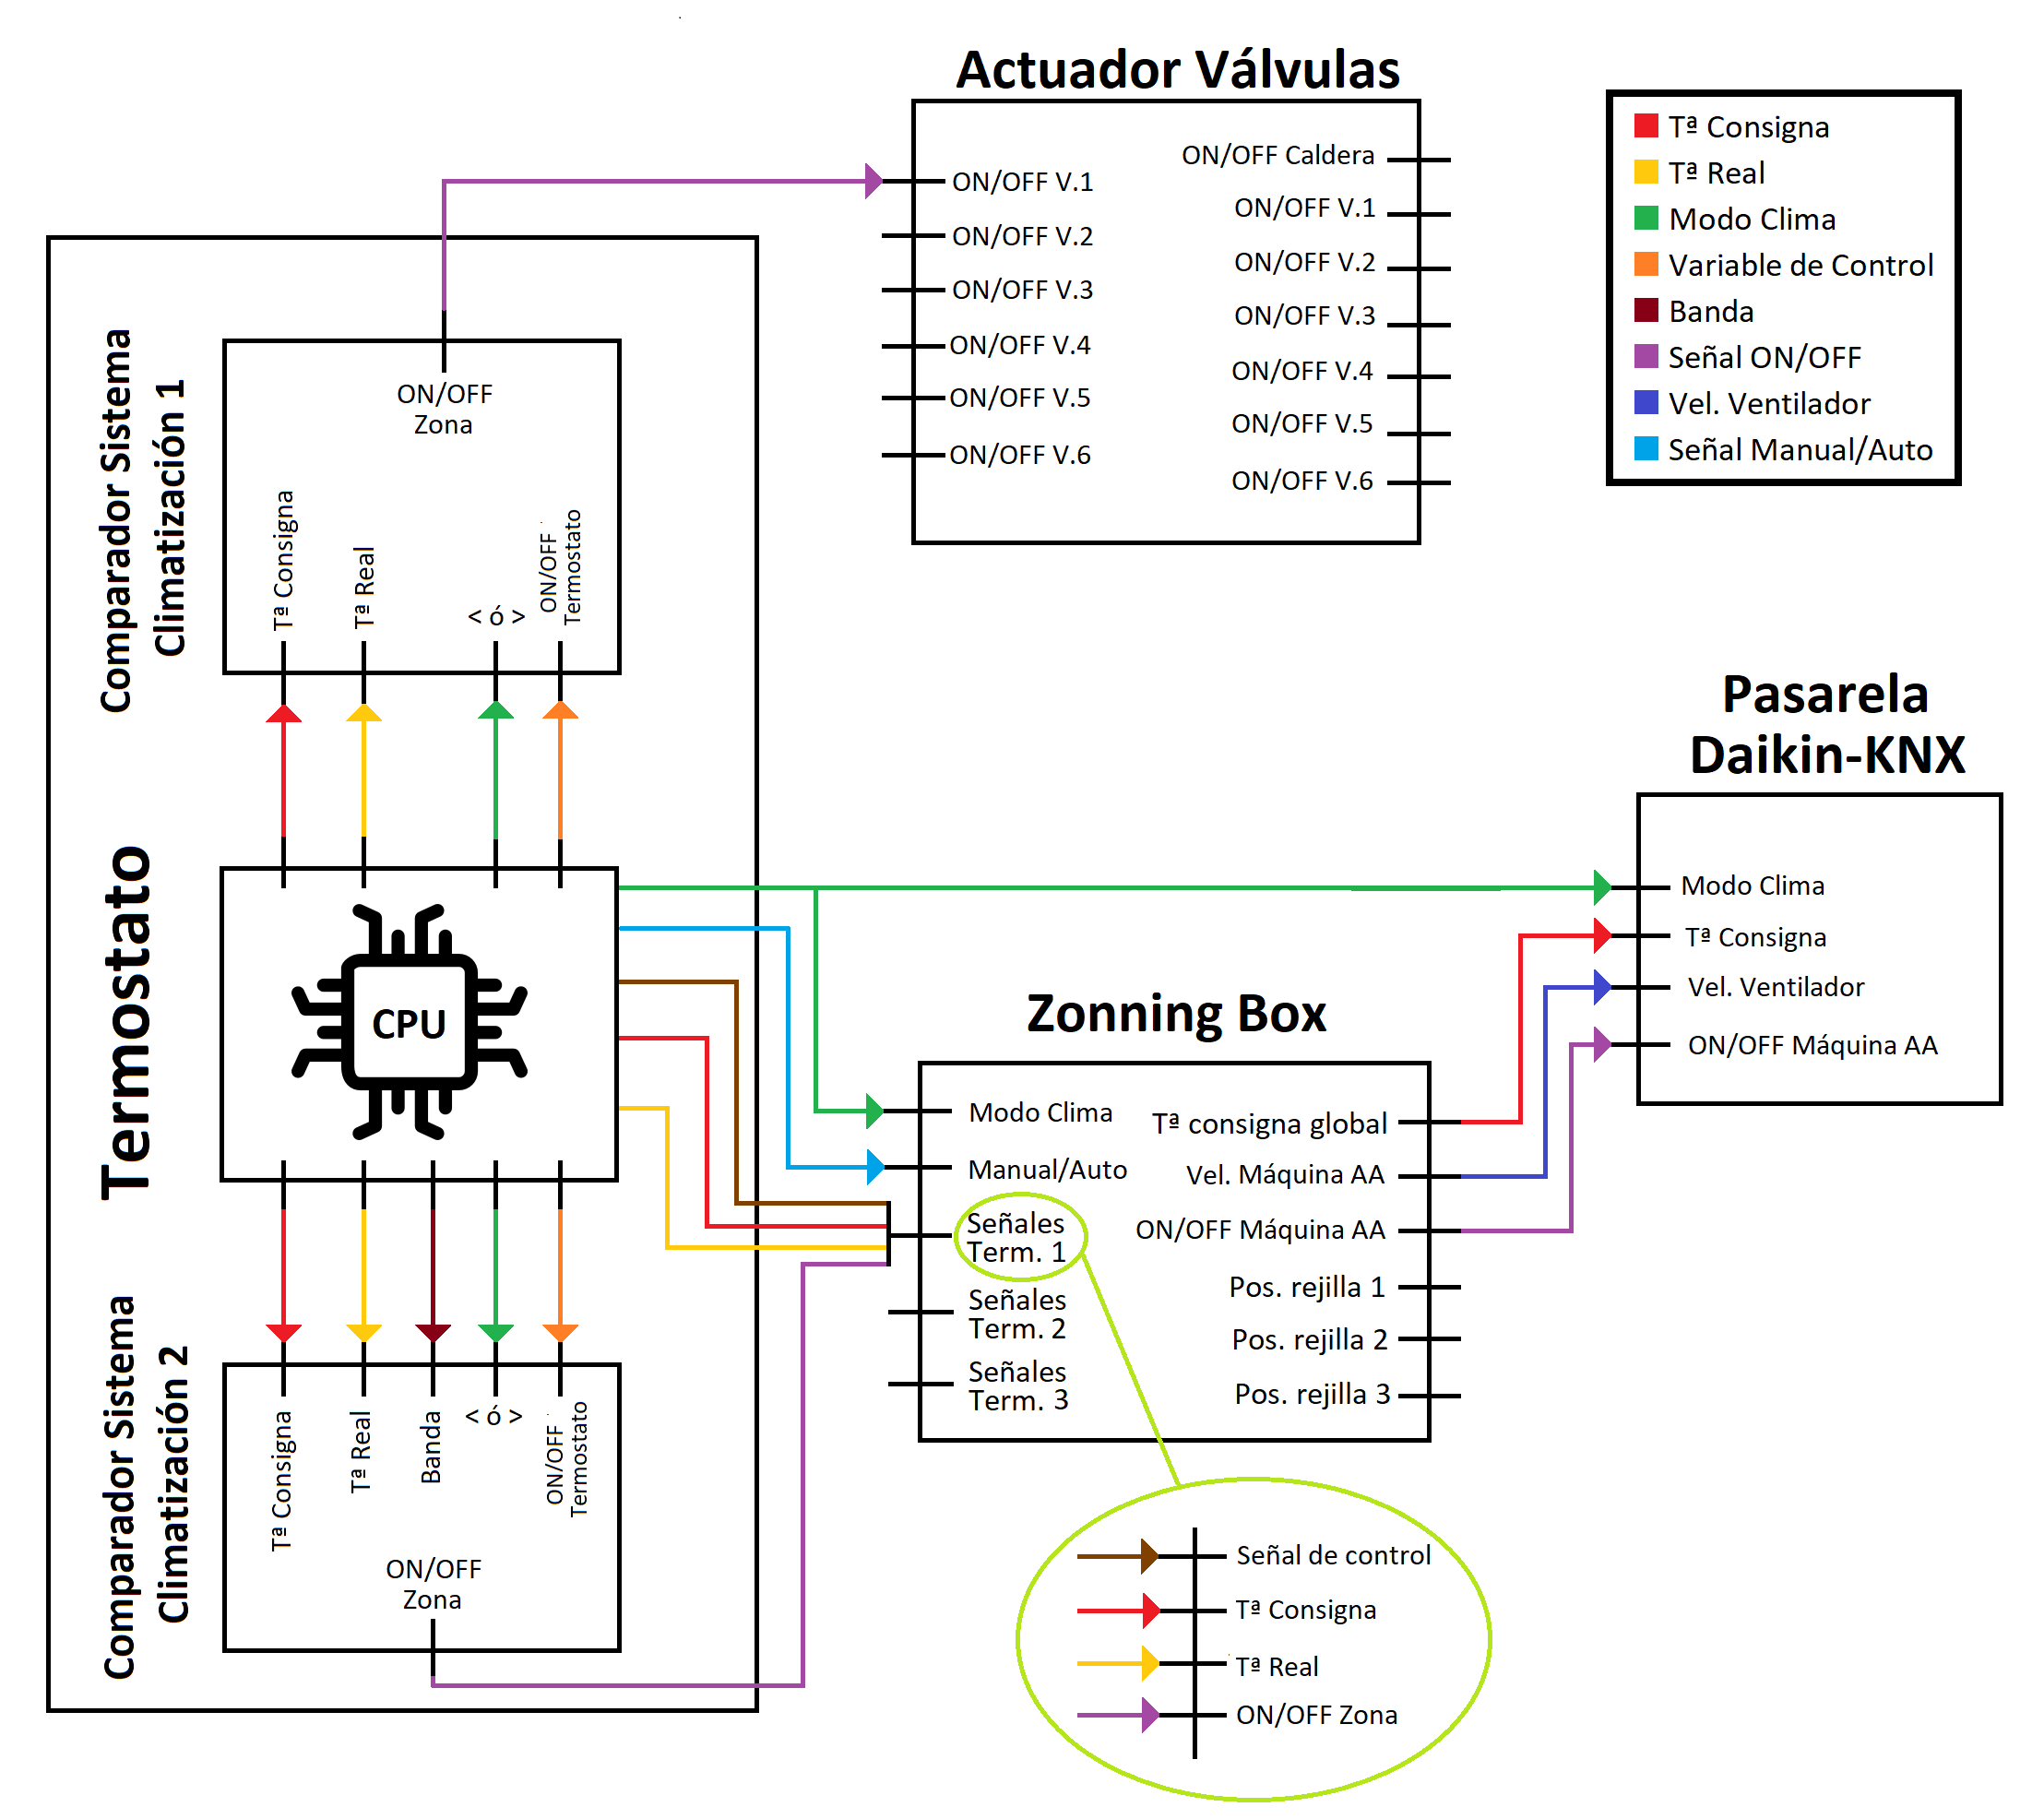
\includegraphics[width=1.15\textwidth]{figures/prog_termost.png}   
\caption{Esquema linkado sistema de climatización}
\label{fig:prog_termost}
\end{figure}
\end{center}
A la izquierda de la Imagen \ref{fig:prog_termost}, aparece uno de los termostatos a instalar en la vivienda. En su interior podemos encontrar su módulo de procesamiento, por el cual recibirá y retransmitirá todas las variables que componen el sistema de climatización enviadas desde la aplicación móvil, el X1 o desde sus propios pulsadores accionados por el cliente. \\Las variables que maneja serán las siguientes: 
\begin{itemize}
\item \textbf{Modo clima:} es el parámetro que indica al sistema si debe actuar controlando la temperatura de la vivienda en modo verano o generador de frio, o por el contrario, lo hará en modo invierno o generando calor. Tendrá un tamaño de 1 bit, asegurando así que el sistema no se encuentre en una situación de dualidad, pudiendo provocar errores o incluso el daño de los equipos de aerotermia. Será seleccionado por el usuario a través de la aplicación o del G1.
\item \textbf{Temperatura real:} será el valor medido de la temperatura de la habitación por el termómetro interno del termostato instalado en ella. Tendrá un tamaño de 2 bytes.
\item \textbf{Temperatura de consigna:} esta variable de 2 bytes reflejará el valor deseado por el cliente de temperatura en una determinada habitación y será seleccionada a través de los pulsadores de cada termostato o bien desde la aplicación o del G1. Como se explicó en la sección \ref{sec:sec_clima}, se ha optado por un control de tipo PI para lograr que la temperatura real logre igualarse a la de consigna.
\item \textbf{Banda:} este parámetro marcará la diferencia de temperatura requerida para que el sistema secundario de climatización comience a actuar en el modo de clima generador de calor. Es decir, si la banda tiene su valor fijado en 3ºC y la temperatura de consigna de la habitación es de 25ºC, la CPU no enviará una señal de encendido si la temperatura real se encuentra por encima de los 22ºC, de igual manera que si el sistema se encuentra muy por debajo de la consigna y pasado el rato supera el límite marcado por la banda, se enviará una señal de desconexión al sistema secundario de aerotermia. Al igual que las variables de temperatura, poseerá un tamaño de 2 bytes.
\item \textbf{Variable de control:} esta señal de 1 byte de tamaño será enviada a los controladores de los equipos de aerotermia indicando el porcentaje de apertura o demanda requerido por el sistema, en función de la magnitud de la diferencia entre las temperaturas real y de consigna de cada estancia.
\item \textbf{Señal de ON/OFF:} se trata de una señal tipo todo/nada, es decir, 1 bit,  que se enviará a los equipos en el momento en que haya demanda de calor o frio en las habitaciones y se cumplan los requisitos ya mencionados anteriormente.
\item \textbf{Modo manual/automático:} esta señal binaria (1bit), permitirá al usuario elegir entre el control manual o automático de los ventiladores del fancoil.
\item \textbf{Velocidad del ventilador:} esta señal, tal y como indica su nombre, marcará la velocidad a la que debe rotar el ventilador de la máquina de fancoil. Será enviada desde el módulo de actuación de rejillas si el usuario tiene seleccionado el modo automático, mientras que por el contrario, si se encuentra activado el modo manual, será el usuario a través de la aplicación o el G1 quien seleccione el nivel de velocidad deseado. Tendrá un tamaño de 1 byte.
\end{itemize}
Estas señales servirán para gobernar el resto de módulos que componen el sistema de climatización: el actuador de rejillas, la pasarela a la máquina de aerotermia y el actuador de las válvulas para cumplir con la funcionalidad detallada en el capítulo \ref{sec:sec_clima}.  Para lograr estos resultados, la programación de cada uno de los  ZonningBox se realizó para el control de 3 zonas cada una con un solo grupo de aerotermia. Al controlarse la entrada de aire a varios habitáculos desde un único controlador, se ha decidido implementar una serie de medidas de seguridad para evitar el daño de los conductos de ventilación y de los equipos, y es que, al cerrarse las rejillas de manera hermética, si la máquina aerogeneradora expulsase aire en el momento en el que todas se encuentran cerradas (tanto al comienzo del proceso de regulación de la temperatura, cuando todas se encuentran cerradas, o bien al finalizar, que las rejillas cerrasen antes de que la máquina cesase de expulsar aire), provocaría un aumento no controlado de la presión del sistema, con la posibilidad de destruir la estanqueidad creada por los técnicos a la hora de la instalación de las máquinas y los conductos. Otra de las medidas instaladas para la prevención y el mantenimiento del buen estado del sistema es la programación de la apertura y cierre automático de las rejillas cuando estas llevan un tiempo prolongado sin utilizarse, una semana, previniendo así el agarrotamiento y la acumulación de polvo en el interior de sus partes mecánicas. Por último se ha medido y programado el tiempo que tardan en abrirse y cerrarse las rejillas para evitar que los motores fuercen y dañen las rejillas o el marco sobre el que se apoyan estas al cerrarse.\\
Por otro lado, y para cumplir con las especificaciones del cliente, se ha programado que el control que realiza el ZonningBox sobre los ventiladores lo realice sobre la posibilidad de regulación de estos en 3 velocidades distintas y que su selección sea elegida o bien por el propio usuario en el modo manual, o bien por el propio ZonningBox haciendo uso de los factores de ponderación que se ha otorgado a cada zona.De manera similar a las rejillas, las válvulas han sido programadas para que se ejecute un cierre controlado y escalado, evitando así la sobrepresión de las tuberías al tratar de forzar la entrada de más agua al sistema de cañerías.\\\\
Estos módulos poseen una programación relativamente sencilla frente a la que tienen los termostatos debido principalmente a la diferencia de roles que adoptan cada uno: mientras que los actuadores de válvulas y rejillas son “esclavos”, los termostatos actúan como “masters” y son quienes generan las variables de control del sistema.\\
Como ya se comentó, este modelo de termostato posee una interfaz con la que el usuario podrá comunicarse con el sistema de climatización a través del uso de la aplicación móvil, la pantalla del G1 o bien desde sus pulsadores y pantallas LED integradas. Estas pantallas LED poseen un modo ahorro en el que se ha configurado que la pantalla muestre la hora del sistema y la temperatura real a la que se encuentra la habitación en la que se ha instalado. Una vez que entran en uso, y por tanto, salen del modo ahorro, estas pantallas se han programado para que muestren el comportamiento de determinados parámetros en paralelo con la funcionalidad que se ha otorgado a los botones, y es que cada uno de los cuatro pulsadores tendrá asociada una porción de pantalla: 
\begin{itemize}
\item \textbf{Cuadrante superior izquierda:} se ha reservado para el control del ON/OFF del termostato. Trabajando con la variable de 1 bit, el usuario podrá activar o desactivar la climatización en esa estancia haciendo uso del pulsador y viendo el estado en que se encuentra sobre la pantalla mediante el uso de un icono de OFF para cuando se encuentre desactivado, o bien por el contrario, mostrando un icono de climatización encendida. 
\begin{figure}[H]
\begin{center}

\includegraphics[width=0.45\textwidth]{figures/iconos_term.png}   
\caption{Iconos de los cuadrante superior izquierda de los termostatos}
\label{fig:iconos_term}
\end{center}
\end{figure}

\item \textbf{Cuadrante superior derecha:} será utilizado para el control de las velocidades del ventilador del aire acondicionado. Desde este pulsador, el cliente podrá seleccionar entre los tres niveles de velocidad preprogramados o el modo automático, pasando por cada uno de ellos con cada pulsación, dando la vuelta de manera cíclica. En la pantalla aparecerá un número para indicar la velocidad del modo manual, o en el caso del modo automático, se mostrará por pantalla la palabra “AUTO”.
\item \textbf{Cuadrantes inferiores:} ambos cuadrantes inferiores se han programado de manera asociada para permitir al usuario el control de la temperatura de consigna: con el pulsador de la izquierda podrá reducir su valor en saltos de 0.2ºC, mientras que por el contrario, con el de la derecha podrá incrementarlo. Los valores que vaya tomando esta variable serán mostrados en su sección de pantalla para un ajuste más controlado.
\begin{figure}[H]
\begin{center}
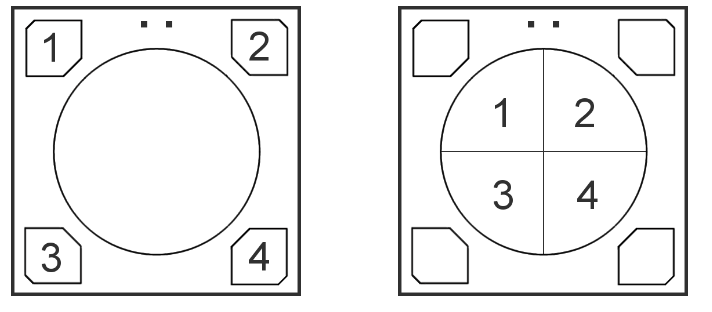
\includegraphics[width=0.75\textwidth]{figures/iconos_term2.png}   
\caption{Representación pulsadores (izq) y pantallas (der) de los termostatos}
\label{fig:iconos_term2}
\end{center}
\end{figure}
\end{itemize}
Al terminar la programación estas serían (Imágenes \ref{fig:prog_clima1} y \ref{fig:prog_clima2}) las variables que han sido utilizadas y linkadas de un termostato,  una máquina de aerotermia, una válvula reguladora de suelo radiante, una rejilla y la caldera. A todas estas habría que sumarle las respectivas variables del resto de elementos que poseen la misma configuración, y por ello han sido omitidas sus programaciones en este documento, ya que, podrían replicarse con los ejemplos mostrados en el Anexo~\ref{aped.B}.

\subsection{Sistemas sensoriales}La programación de los sistemas sensoriales, a excepción del recuperador de CO\textsubscript{2}, se basa en la transmisión del estado en que se encuentra en cada momento el sensor asociado al módulo de entradas, para que el resto de módulos actúen en consecuencia a la lógica con la que han sido programados.\\
Un ejemplo de esto lo podemos ver en la programación del sensor de presencia en la Imagen \ref{fig:prog_pres}, en la que podemos ver que actúa sobre cierta luminaria, controlando sus variables de encendido y regulación. Se ha configurado para que sus tres zonas PIR actúen al unísono, logrando así un barrido de 360º de la estancia con un modo de funcionamiento automático, permitiendo la conexión y desconexión de la luz de manera autónoma. En cuanto a los valores  limites, se ha determinado un valor de 1000 luxes como valor límite del umbral inferior de manera empírica, por lo que, si la detección es inferior a este valor, la luminaria no se encendería, ahorrando así energía en los momentos del día en que es suficiente iluminación con la luz natural.
La programación de los sensores de movimiento podemos verla en la Imagen \ref{fig:prog_mov}, en la que únicamente actúan sobre la señal ON/OFF, siguiendo la funcionalidad otorgada a la hora del diseño. Para ellos, se han asociado sus dos sectores PIR que poseen, y al igual que los sensores de presencia, tramitarán la conexión y la desconexión de manera autónoma con un umbral límite de 1000 luxes.\\
El detector de humo también poseerá una programación sencilla, tal y como podemos ver en la Imagen \ref{fig:prog_humo}.  Poseerá dos variables diferentes para poder distinguir si la alarma ha sido saltada por la presencia de humos, o bien por un aumento drástico de la temperatura, detectada por el sensor termovelocimétrico. Ambas detecciones actuarán sobre la salida del actuador asociada con la sirena de emergencia.\\
Por último, los sensores de inundación y ventana abierta, se han programado trabajando con la detección de las variaciones de flanco, tal y como lo haría un módulo de entradas corriente. Enviarán las señales de alarma una vez que o bien el agua o el cierre magnético logren cerrar el circuito y generen un flanco de subida sobre alguna de las entradas de sus respectivos módulos. Podemos ver su programación en las Imágenes \ref{fig:prog_inun} y \ref{fig:prog_vent}.

\subsection{Recuperador de CO\textsubscript{2}}


\subsection{Control de consumos}


\subsection{Escenas y centralizados}Como ya se comentó en la Sección \ref{sec:dir_grup}, las escenas y centralizados se tratan de direcciones de grupos que permiten ejecutar una rutina de eventos atacando un único objeto de comunicación, teniendo como principal diferencia que las escenas permitían enviar parámetros con valores distintos tanto en valor como en tipado, mientras que los centralizados no, siendo enviado exactamente el mismo valor a todas las direcciones asociadas. En añadido, las escenas tendrán una programación diferente a la que poseerán los centralizados, los cuales solo deben tener las direcciones de grupo linkadas. Las escenas funcionan enviando un número del 1 al 255 indicando así cuál de todas será ejecutada, siendo cada uno de estos números la identificación utilizada para escogerlas. Por tanto, cada salida del actuador que se desee que participe en una escena, deberá tener activada la opción de generar escenas, tener programada su acción durante la ejecución de la escena y atribuido su número identificador. A continuación se exponen algunas de estas direcciones de grupo especiales:
\begin{itemize}
\item Salir de casa: en esta escena se han enlazado señales de persianas y luminarias, enviando una señal de OFF a todas las salidas de los actuadores conectados a una bombilla y una señal de DOWN a las salidas asociadas a las persianas. Será utilizada para que el cliente pueda salir de su casa con la convicción de no haberse dejado ninguna de las luces encendidas y sienta cierto tipo de seguridad al saber todas las persianas han sido bajadas, sobre todo en viviendas de tipo unifamiliar.
\item Vacaciones: en esta escena se combina la escena “Salir de casa” con el apagado de todo el equipo de climatización, permitiendo al cliente el apagado de la caldera, los equipos de aerotermia y el suelo radiante a la vez que el cierre de las válvulas y rejillas de la vivienda.
\item Buenos días: las ordenes que se ejecutan en esta escena tienen como misión la de añadir un plus de confort a la instalación, permitiendo al usuario que con un salo click o programando un temporizador, las persianas de toda la casa se sitúen en una posición concreta que permita entrar la luz del sol justa a la casa, a la vez que se encienden ciertas luces de la casa con una intensidad determinada.
\item Cine: esta escena está especialmente diseñada para la habitación en la que se instalará un proyector, simulando crear una pequeña sala de cine en la vivienda. Esta escena permitirá ambientar la estancia con un único click, regulando la posición de las persianas y la intensidad de la luz, a la vez que se despliega la pantalla donde será proyectada la película.
\end{itemize}

\subsection{Sistemas de visualización y protocolo de comunicación}